\documentclass[aspectratio=64,11pt]{beamer}
\usepackage{graphicx}
\usepackage{longtable}
\usepackage{wrapfig}
\usepackage{rotating}
\usepackage[normalem]{ulem}
\usepackage{amsmath}
\usepackage{amssymb}
\usepackage{capt-of}
\usepackage{hyperref}
\institute{Università di Siena}
\usepackage{localheader}
\usepackage{tikz}
\usepackage{booktabs}
\usepackage{setspace}
\usepackage{quoting}
\usepackage[italian]{babel}
\usepackage{fancybox}
\usetheme{default}
\author{Massimo D'Antoni}
\date{2023-2024}
\title{I limiti dell'azione pubblica: \newline i problemi delle scelte collettive}
\subtitle{Scienza delle Finanze}
\hypersetup{
 pdfauthor={Massimo D'Antoni},
 pdftitle={I limiti dell'azione pubblica: i problemi delle scelte collettive},
 pdflang={Italian}}
\begin{document}

\maketitle


%%%%%%%%%%%%%%%%%%%%%%%%%%%%%%%%%%%%%%%%
\begin{frame}{I limiti dell'azione pubblica}
\begin{itemize}
\item Finora abbiamo considerato casi nei quali il mercato "fallisce" l'obiettivo
di fornire beni e servizi in modo efficiente:
\begin{itemize}
\item esternalità
\item beni pubblici
\item beni forniti in condizioni di monopolio
\item fallimenti dei mercati assicurativi
\item previdenza e pensioni
\end{itemize}
\item Ma lo stato è effettivamente in grado di supplire a questi limiti del mercato?
\begin{itemize}
\item Come si determinano le azioni pubbliche?
\item Cosa spinge lo Stato ad agire nell'interesse dei cittadini?
\item Anche quando gli obiettivi dello Stato siano ben orientati, avrà esso la
capacità di realizzare tale obiettivi? Es. ha le informazioni necessarie?
\end{itemize}
\item Ci occupiamo del primo aspetto: le decisioni collettive
\end{itemize}
\end{frame}

\section{L'accordo unanime\newline nella fornitura di un bene pubblico}

%%%%%%%%%%%%%%%%%%%%%%%%%%%%%%%%%%%%%%%%
\begin{frame}{Lo Stato come contratto}
\begin{itemize}
\item In un contratto le parti si vincolano a compiere certe azioni e si possono
prevedere sanzioni per il mancato adempimento
\item L'accettazione degli obblighi è collegata all'adesione volontaria degli
individui, che stipulano il contratto nel mutuo interesse
\item Idea dello Stato come contratto già in filosofi come Thomas Hobbes, John
Locke, Jean-Jacques Rousseau e Immanuel Kant
\item Più tardi, la visione dello «scambio volontario» di Knut Wicksell
(1851-1926), ma anche esponenti della scuola italiana di scienze delle
finanze come Antonio De Viti De Marco (1858-1943) e della \emph{public choice}
come James Buchanan (1919-2013).
\item Caratteristica del contratto è l'adesione volontaria dei contraenti:
l'unanimità.
\item Approccio dello \emph{scambio volontario}:
\begin{itemize}
\item Rapporto cittadino/stato visto come uno scambio
\item Decisione sull'erogazione dei beni pubblici presa all'\alert{unanimità}
\end{itemize}
\end{itemize}
\end{frame}

%%%%%%%%%%%%%%%%%%%%%%%%%%%%%%%%%%%%%%%%
\begin{frame}{L'unanimità}
\begin{itemize}
\item Perché una decisione sia unanime occorre che l'esito determini un
miglioramento paretiano (condizione necessaria, ma non sufficiente).
\item L'unanimità implica la necessità di un compromesso mutuamente vantaggioso
tra i partecipanti.
\item Tuttavia, nell'ambito di un miglioramento paretiano, il «surplus» può essere
ripartito in molti modi.
\item Gli individui possono utilizzare il proprio potere di veto per influenzare
la ripartizione del surplus, a scapito del raggiungimento di un
accordo. L'accordo non è scontato.
\end{itemize}
\end{frame}

%%%%%%%%%%%%%%%%%%%%%%%%%%%%%%%%%%%%%%%%
\begin{frame}{Il meccanismo di Lindahl}
\begin{itemize}
\item Nell'idea di Lindahl, un procedimento simile al mercato in grado di
determinare una decisione unanime
\begin{itemize}
\item un «banditore» che propone con prezzi personalizzati (ipotesi: costo
marginale del bene pubblico costante $p$)
\item quota/prezzo a carico dell'individuo $h$ è indicata da $\tau_h$, con
$0\le\tau_h\le1$ e $\sum_h\tau_h=1$
\item quantità desiderata da $h$ è data da $\text{BM}^{h}(Y)=\tau_hp$
\item quando le quantità desiderate coincidono raggiungiamo l'equilibrio
\item se esse non coincidono si modificano i prezzi (si abbassa $\tau_h$ per gli
$h$ che desiderano una quantità minore\dots{})
\item In equilibrio $\sum_h\text{BM}^{h}(Y^*)=p$, si raggiunge la quantità
efficiente
\end{itemize}
\end{itemize}
\end{frame}
%%%%%%%%%%%%%%%%%%%%%%%%%%%%%%%%%%%%%%%%
\begin{frame}{Meccanismo di Lindahl}
\begin{columns}
\begin{column}{.5\columnwidth}
Illustrazione grafica con due individui:
\begin{itemize}
\item Si parte con le quote $\bar\tau_1$ e $\bar\tau_2$, in corrispondenza delle
quali l'individuo 1 domanda una quantità maggiore dell'individuo 2
\item Si correggono le quote fino a raggiungere $\tau_1^*$ e $\tau_2^*$ dove le
quantità desiderate coincidono
\end{itemize}
\end{column}
\begin{column}{.5\columnwidth}
\begin{figure}[htbp]
\centering
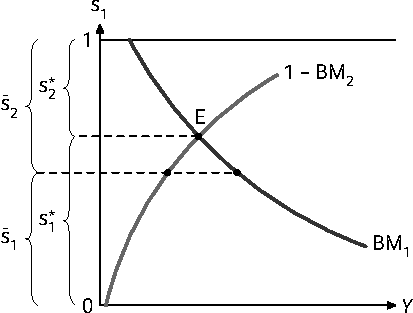
\includegraphics[width=\textwidth]{./figure/lindahl-1.pdf}
\end{figure} 
\end{column}
\end{columns}
\end{frame}
%%%%%%%%%%%%%%%%%%%%%%%%%%%%%%%%%%%%%%%%
\begin{frame}{Meccanismo di Lindahl: comportamento strategico}
\begin{columns}
\begin{column}{.5\columnwidth}
Nell'ipotesi che l'individuo 1 si comporti in modo strategico, rappresentando
le proprie preferenze in modo non sincero:
\begin{itemize}
\item "Simulando" una domanda inferiore ($\tilde v_1$) e portandosi in F,
l'individuo 1 ottiene un livello di utilità maggiore
\item tale comportamento determina una perdita di efficienza
\end{itemize}
\end{column}
\begin{column}{.5\columnwidth}
\begin{figure}[htbp]
\centering
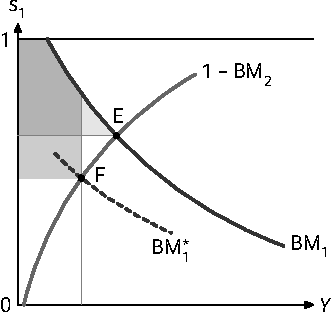
\includegraphics[width=\textwidth]{./figure/lindahl-2.pdf}
\end{figure} 
\end{column}
\end{columns}
\end{frame}
%%%%%%%%%%%%%%%%%%%%%%%%%%%%%%%%%%%%%%%%
\begin{frame}{Meccanismo di Lindahl: comportamento strategico}
\begin{columns}
\begin{column}{.5\columnwidth}
Se entrambi gli individui si comportano in modo strategico:
\begin{itemize}
\item l'esito sarà un punto come G, in cui la quantità prodotta è inferiore a
quella efficiente ed entrambi gli individui stanno peggio rispetto ad E
\item la soluzione di Lindahl non è immune dal problema del \emph{free riding}: gli
individui tenderanno a sottostimare il beneficio per ottenere un vantaggio
in termini di contributo alla produzione di bene pubblico
\end{itemize}
\end{column}

\begin{column}{.5\columnwidth}
\begin{figure}[htbp]
\centering
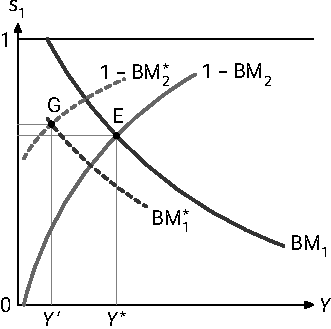
\includegraphics[width=\textwidth]{./figure/lindahl-3.pdf}
\end{figure} 
\end{column}
\end{columns}
\end{frame}

%%%%%%%%%%%%%%%%%%%%%%%%%%%%%%%%%%%%%%%%
\begin{frame}{Perché la negoziazione può finire male}
\begin{itemize}
\item Consideriamo due individui che devono decidere come ripartire il costo di un
bene (120).
\item Il primo individuo, che valuta il bene 200, non sa se per il secondo
individuo il bene vale 100 oppure 50. Attribuisce alla prima possibilità una
probabilità del 75\%.
\item Il primo individuo può formulare una proposta «prendere o lasciare» al
secondo individuo:
\begin{itemize}
\item se propone una ripartizione $(20,100)$, la proposta è accettata con
probabilità 75\% e il primo individuo guadagna $0,75\cdot(100-20) + 0,25
    \cdot 0 = 60$.
\item se propone $(70,50)$, la proposta è accettata con probabilità 100\% e il
primo individuo guadagna $100-70=30$
\end{itemize}
\item Proponendo $(20,100)$, con probabilità 25\% il bene non verrà prodotto anche
se la produzione sarebbe efficiente.
\end{itemize}
\end{frame}

\section{Maggioranza}


%%%%%%%%%%%%%%%%%%%%%%%%%%%%%%%%%%%%%%%%
\begin{frame}{La maggioranza}
\begin{itemize}
\item Con l'unanimità non è possibile affrontare questioni redistributive e in
generale giochi «a somma zero» o questioni relative a benefici non
divisibili.
\item Anche in presenza di un surplus, il raggiungimento di un accordo unanime può
richiedere negoziazioni estenuanti e c'è la possibilità che l'accordo non
sia raggiunto
\item Un modo per ridurre tali costi è quello di decidere \alert{a maggioranza}
\item La maggioranza presenta tuttavia alcune controindicazioni:
\begin{itemize}
\item rischio che una maggioranza prevarichi su una minoranza, infliggendo
perdite rispetto allo \emph{status quo};
\item non tenendo conto dell'intensità delle preferenze, le perdite della
minoranza possono facilmente eccedere i benefici per la maggioranza: non è
garantito che una decisione a maggioranza comporti una maggiore efficienza
potenziale.
\end{itemize}
\item Inoltre, date le preferenze individuali, la maggioranza non sempre dà luogo
a una scelta univoca.
\end{itemize}
\end{frame}

%%%%%%%%%%%%%%%%%%%%%%%%%%%%%%%%%%%%%%%%
\begin{frame}{Il paradosso del voto a maggioranza}
\begin{itemize}
\item In presenza di più di dua alternative:
\begin{itemize}
\item accontentandoci della \alert{maggioranza relativa} potremmo selezionare
un'alternative che risulterebbe perdente in un confronto diretto rispetto
a un'altra opzione;
\begin{equation*}
\text{I:}\enspace a \succ b \succ c \qquad 
\text{II:}\enspace b \succ a \succ c \qquad 
\text{III:}\enspace c \succ a \succ b.
\end{equation*}
\item richiedendo che l'opzione scelta sia preferita a maggioranza rispetto a
\emph{qualsiasi} opzione alternativa (criterio di Condorcet), potremmo non
essere in grado di selezionare un'alternativa preferita
L'ordinamento che emerge dal voto a maggioranza tra coppie di alternative
è \alert{ciclico}!
\begin{equation*}
\text{I:}\enspace a \succ b \succ c \qquad 
\text{II:}\enspace b \succ c \succ b \qquad 
\text{III:}\enspace c \succ a \succ b.
\end{equation*}
\end{itemize}
\item Si tratta del \alert{paradosso del voto a maggioranza}, o \alert{paradosso di Condorcet}
\item È una situazione frequente quando si debba decidere a maggioranza
come suddividere i benefici/costi di una decisione
\end{itemize}
\end{frame}

%%%%%%%%%%%%%%%%%%%%%%%%%%%%%%%%%%%%%%%%
\begin{frame}{Elettore mediano e preferenze unimodali}
\begin{itemize}
\item Il paradosso del voto non si presenta e l'identificazione dell'esito del
voto a maggioranza è agevole quando le preferenze di tutti gli individui
coinvolti sono \alert{unimodali}
\item \alert{Preferenze unimodali}: l'individuo considera via via meno desiderabili
alternative che si allontano da quella preferita
\end{itemize}
\begin{columns}
\begin{column}{.5\columnwidth}
\begin{figure}[htbp]
\centering
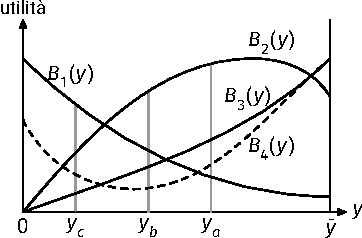
\includegraphics[width=\textwidth]{./figure/elettore-mediano-1.pdf}
\end{figure}
\end{column}
\begin{column}{.5\columnwidth}
\begin{figure}[htbp]
\centering
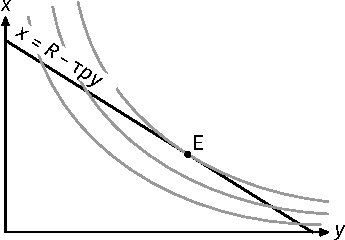
\includegraphics[width=\textwidth]{./figure/elettore-mediano-3.pdf}
\end{figure}
\end{column}
\end{columns}
\end{frame}


%%%%%%%%%%%%%%%%%%%%%%%%%%%%%%%%%%%%%%%%
\begin{frame}{Elettore mediano e preferenze unimodali /2}
\begin{block}{Teorema dell'elettore mediano}
Se le preferenze sono unimodali, e le alternative preferite sono ordinabili
 su una dimensione, la scelta ricadrà sull'alternativa preferita
 dell'\emph{elettore mediano} (rincorsa verso il "centro")
\end{block}

\begin{columns}
\begin{column}{.5\columnwidth}
Una collettività di 7 individui con preferenze unimodali.
\medskip

\begin{tabular}[c]{ll}
  2 individui considerano ottimale&\emph{A}\\
  3 individui considerano ottimale&\emph{B}\\
  un individuo considera ottimale &\emph{C}\\
  2 individui considerano ottimale &\emph{D}\\
  4 individui considerano ottimale &\emph{E}\\
  un individuo considera ottimale &\emph{F}
\end{tabular}
\end{column}

\begin{column}{.5\columnwidth}
\begin{figure}[htbp]
\centering
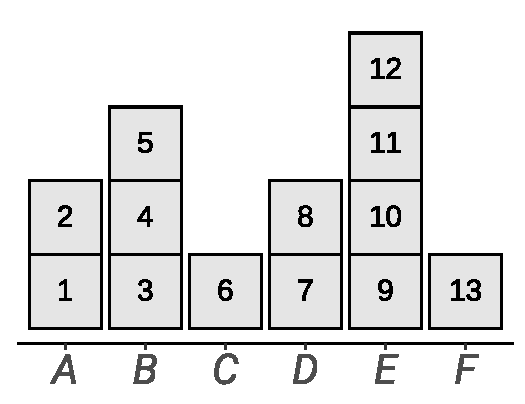
\includegraphics[width=.8\textwidth]{./figure/elettore-mediano-distribuzione.pdf}
\end{figure}

L'alternativa selezionata sarà D, la preferita dell'individuo 7, che rappresente l'elettore mediano.
\end{column}
\end{columns}
\end{frame}

%%%%%%%%%%%%%%%%%%%%%%%%%%%%%%%%%%%%%%%%
\begin{frame}{Preferenze unimodali}
\begin{itemize}
\item Esempi di preferenze non unimodoli (preferenza per gli estremi) nel caso di
decisioni su un'unica dimensione: risorse investite in una certa azione
militare, finanziamento dell'istruzione pubblica ecc.
\end{itemize}

\begin{columns}
\begin{column}{.5\columnwidth}
\scriptsize
«Chiedo al Congresso e al paese di accettare un fermo impegno a un nuovo programma di azione, un programma che durerà per molti anni e comporterà costi pesanti: 531 milioni di dollari nel bilancio nel 1962, un aumento stimato dai sette ai nove miliardi di dollari nei prossimi cinque anni. Se dobbiamo fermarci a metà o ridimensionare i nostri obiettivi di fronte alle difficoltà, a mio giudizio è meglio non iniziare neppure.»
\vspace{3mm}

[Discorso al Congresso del 25/5/1961]
\end{column}

\begin{column}{.5\columnwidth}
\begin{figure}[htbp]
\centering
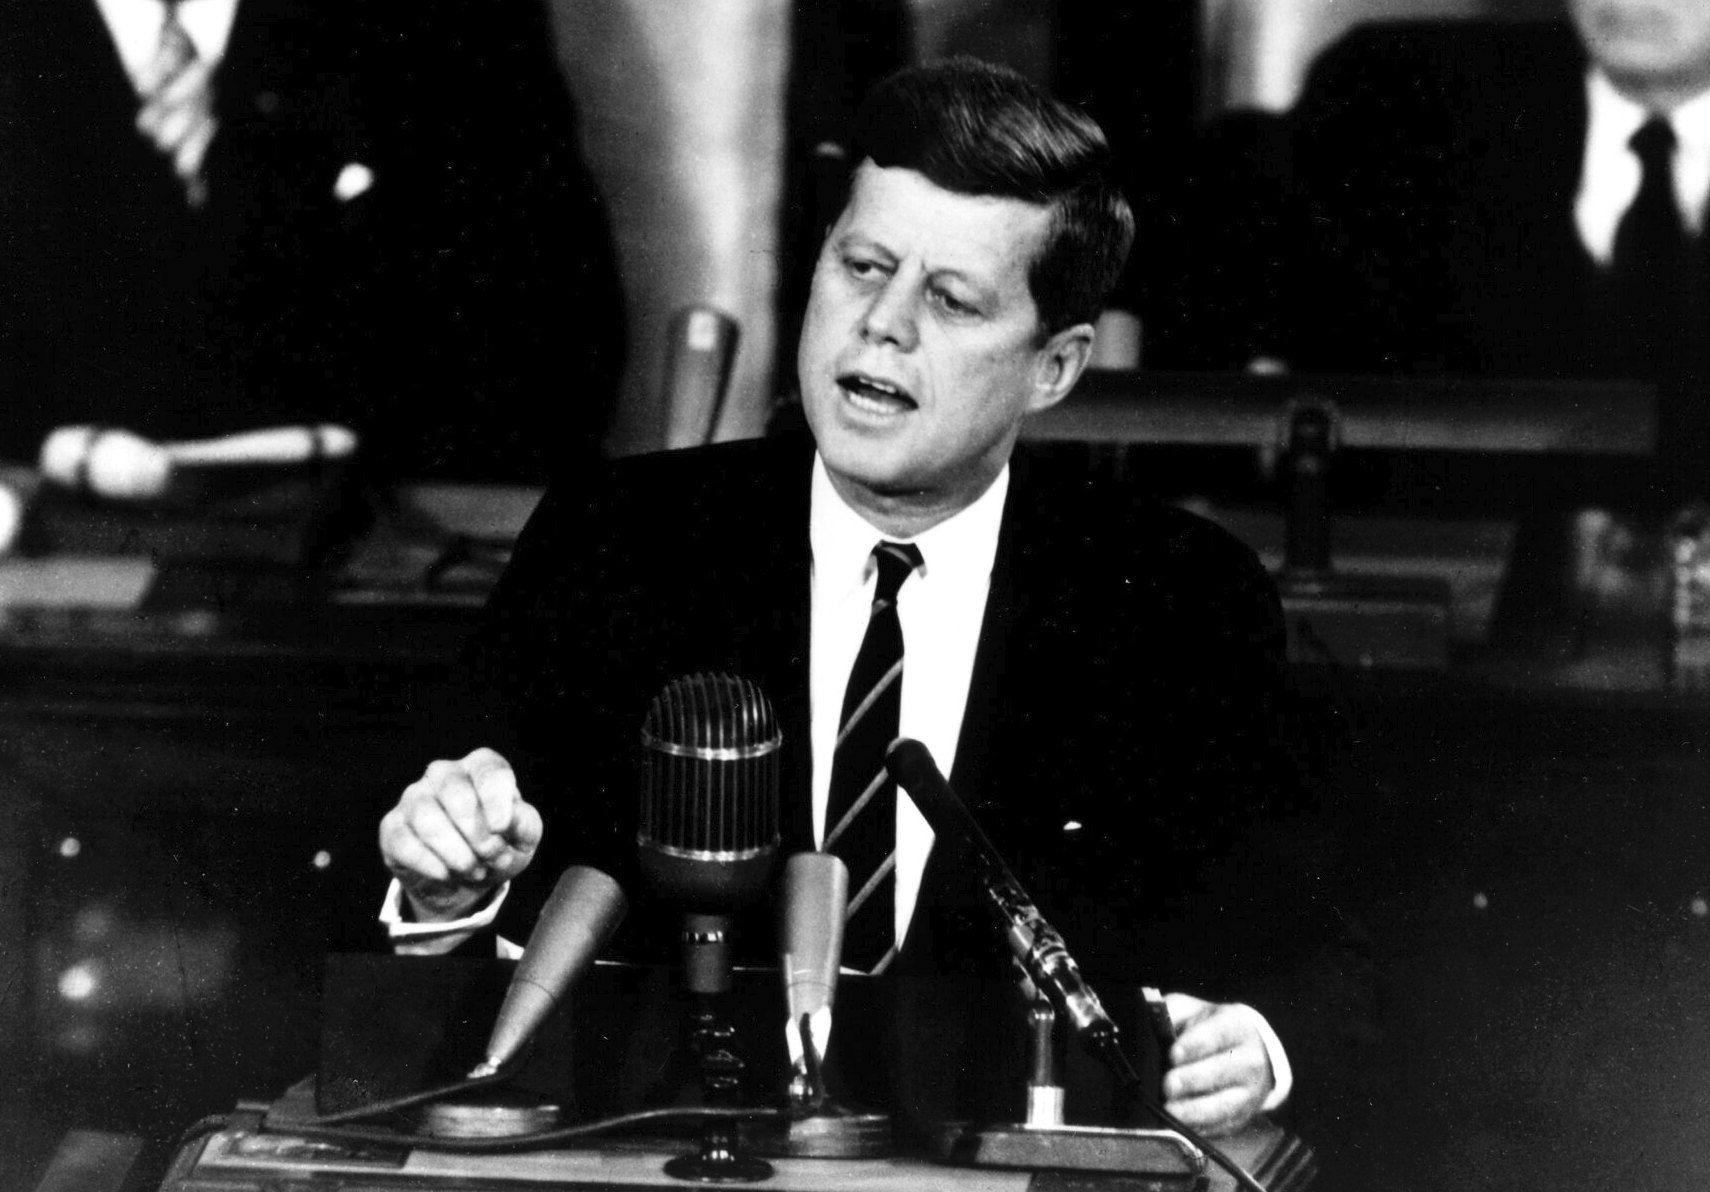
\includegraphics[width=\textwidth]{./figure/John-Kennedy-NASA.jpg}
\end{figure}
\end{column}
\end{columns}
\end{frame}

%%%%%%%%%%%%%%%%%%%%%%%%%%%%%%%%%%%%%%%%
\begin{frame}{Alcune varianti del voto a maggioranza}
\begin{itemize}
\item Visto che non sempre possiamo escludere la presenza di cicli, al fine di
evitare che la mancanza di un'alternativa vincente su tutte le altre porti ad
un'impasse decisionale, si adottano procedure che consentono di raggiungere
comunque una decisione:
\begin{itemize}
\item \alert{Plurality rule (maggioranza relativa)}: vince l'opzione che ha avuto più
voti, anche senza maggioranza assoluta
\item \alert{Doppio turno con ballottaggio:} se nessuno ottiene la maggioranza, si
effettua il voto di ballottaggio tra i due candidati con più voti
\item \alert{Voto multiplo:} ciascuno indica più di un'alternativa preferita e si
adotta quella che ha avuto più voti
\item \alert{Voto con scarto:} si scarta l'alternativa che ha ottenuto meno voti o, in
alternativa, si chiede di indicare l'alternativa peggiore e si scarta
quella più «votata».
\end{itemize}
\end{itemize}
\end{frame}

%%%%%%%%%%%%%%%%%%%%%%%%%%%%%%%%%%%%%%%%
\begin{frame}{L'esito dipende dal meccanismo scelto}
\begin{center}
  \begin{tabular}{lcc}\toprule
  Gruppo & Numerosità &Preferenze\\
  \midrule
  di sinistra & 15 & $a \succ b \succ c$ \\
  di centro & 14 & $b \succ c \succ a$\\
  di destra & 16 & $c \succ a \succ b$\\\bottomrule
  \end{tabular}
\end{center}

\begin{itemize}
\item Con la maggioranza relativa $c\succ a\succ b$
\item Con il voto multiplo (2 opzioni) abbiamo $a\succ c\succ b$
\item Con il ballottaggio vince $c$
\end{itemize}
Ma è anche possibile che nel caso del ballottaggio una parte di elettori «di
sinistra» converga su $b$ (voto strategico)
\end{frame}

%%%%%%%%%%%%%%%%%%%%%%%%%%%%%%%%%%%%%%%%
\begin{frame}{L'esito è modificato dal «voto strategico»}
\begin{columns}
\begin{column}{.7\columnwidth}
\begin{tabular}{lcc}\toprule
Gruppo & Numerosità &Preferenze\\
\midrule
di sinistra & 15 & $a \succ b \succ c$ \\
di centro-sinistra & 8 & $b \succ a \succ c$ \\
di centro-destra & 6 & $b \succ c \succ a$ \\
di destra & 16 & $c \succ b \succ a$ \\\bottomrule
\end{tabular}
\end{column}

\begin{column}{.3\columnwidth}
\begin{center}
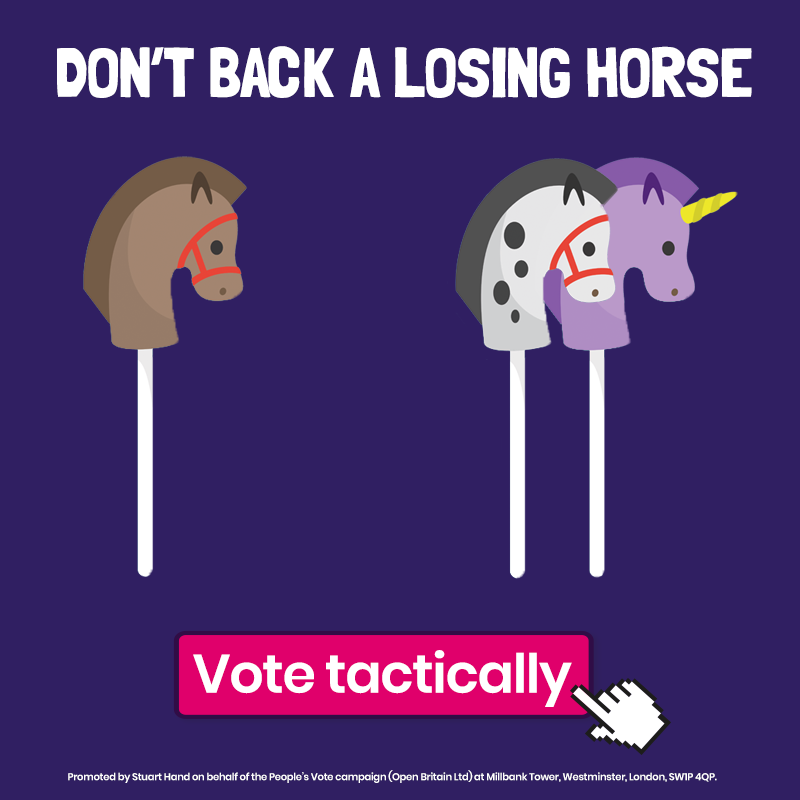
\includegraphics[width=3.3cm]{./figure/vote-tactically.png}
\end{center}
\end{column}
\end{columns}
\end{frame}

%%%%%%%%%%%%%%%%%%%%%%%%%%%%%%%%%%%%%%%%
\begin{frame}{Il meccanismo di voto per punti di Borda}
\begin{center}
\begin{tabular}{lcc}\toprule
  gruppo & numerosità &preferenze\\
  \midrule
  di sinistra & 8 & $a \succ b \succ c\succ d$ \\
  di centro & 12 & $a \succ b \succ d\succ c$ \\
  di destra & 10 & $b \succ c \succ d\succ a$ \\\bottomrule
\end{tabular}
\end{center}

\begin{itemize}
\item Garantisce una scelta, ma
\item tale scelta può non essere Condorcet-vincente
\item il meccanismo è vulnerabile al voto strategico
\end{itemize}
\end{frame}

%%%%%%%%%%%%%%%%%%%%%%%%%%%%%%%%%%%%%%%%
\begin{frame}{L'inefficienza del voto a maggioranza}
\begin{center}
\begin{tabular}{lcccccc}\toprule
    gruppo& numerosità &$a$ &$b$\\
    \midrule
    I      & 3 & 40 & 30\\
    II     & 2 & 40 & 30\\
    III    & 4 & 30 & 60\\\midrule
    \multicolumn{2}{r}{beneficio totale:} & 320 & 390\\
    \bottomrule
\end{tabular}
\end{center}

\begin{itemize}
\item Decisione sulla realizzazione di un bene pubblico (es. un parcheggio)
\item il voto a maggioranza non seleziona la soluzione che massimizza i benefici aggregati
\end{itemize}
\end{frame}

%%%%%%%%%%%%%%%%%%%%%%%%%%%%%%%%%%%%%%%%
\begin{frame}{Scambio di voti}
\begin{center}
\begin{tabular}{lcccccc}\toprule
    gruppo& numerosità &$a$ &$b$ &&$b'$ &$b''$\\
    \midrule
    I      & 3 & 40 & 30 && 30 & 38\\
    II     & 2 & 40 & 30 && 50 & 30\\
    III    & 4 & 30 & 60 && 50 & 54\\\midrule
    \multicolumn{2}{r}{beneficio totale:} & 320 & 390 &&390 & 390\\
    \bottomrule
\end{tabular}
\end{center}

\begin{itemize}
\item Possibile combinare diverse proposte e accordarsi per appoggiarsi reciprocamente: parcheggio con parco giochi o con centro commerciale
\item Lo scambio di voti è un modo per tenere conto dell'intensità delle prefernze e avvicinarsi all'efficienza
\item Ma l'esito finale rischia di essere indeterminato!
\end{itemize}
\end{frame}

%%%%%%%%%%%%%%%%%%%%%%%%%%%%%%%%%%%%%%%%
\begin{frame}{Tirando le somme}
\begin{itemize}
\item Un insieme di scelta troppo ampio (es. con la possibilità di aggiungere
nuove alternative), pur consentendo di avvicinarsi a un esito efficiente,
può determinare instabilità nelle possibili maggioranze e indeterminatezza
dell'esito.
\item La ciclicità dell'esito può essere eliminata o limitata imponendo una
\emph{stopping rule} o adottando i sistemi di voto più complessi in precedenza
descritti, ma questo non assicura l'efficienza, incoraggia il voto
strategico e la manipolazione della procedure decisionale.
\item Limitando l'insieme delle scelte (es. rendendole unidimensionali) alcuni
problemi si risolvono, ma risulta meno probabile il raggiungimento di un
esito efficiente.
\item Anche la maggioranza è segnata dunque da limiti seri!
\end{itemize}
\end{frame}

\section{Il teorema di impossibilità di Arrow}

%%%%%%%%%%%%%%%%%%%%%%%%%%%%%%%%%%%%%%%%
\begin{frame}{Teorema di impossibilità di Arrow /1}
\begin{itemize}
\item È possibile affrontare il problema in termini più generali: invece di
analizzare i problemi di ciascun meccanismo, imponiamo dei requisiti e
individuiamo quali meccanismi li soddisfino (approccio assiomatico).
\item \alert{Regola di scelta sociale}: un procedimento che, a partire dalle preferenze
degli individui, individua un ordinamento delle preferenze
collettivo. Imponiamo delle condizioni:
\begin{itemize}
\item deve produrre un ordinamento, cioè confrontare in modo coerente qualsiasi
coppia di alternative (no ciclicità);
\item deve ssere coerente con il \alert{principio di Pareto}: se un'alternativa è
unanimemente preferita, deve essere socialmente preferita;
\item deve identificare un ordinamento tra le alternative qualunque sia il
profilo di preferenze degli individui (condizione di \alert{universalità} del
dominio);
\item l'ordinamento tra due alternative deve dipendere esclusivamente da come
gli individui ordinano quelle due alternative 
(\alert{indipendenza dalle alternative irrilevanti}).
\end{itemize}
\end{itemize}
\begin{block}{Teorema di impossibilità di Arrow (1951)}
L'unica soluzione compatibile con tutte le condizioni indicate è quella
"dittatoriale", in cui la preferenze di un individuo prevalgono sempre sulle
preferenze di tutti gli altri.
\end{block}
\end{frame}

%%%%%%%%%%%%%%%%%%%%%%%%%%%%%%%%%%%%%%%%
\begin{frame}{L'indipendenza dalle alternative irrilevanti}
\begin{block}{Indipendenza dalle alternative irrilevanti}
La scelta tra due alternative ($a$ e $b$) deve dipendere \alert{soltanto} dal modo
in cui gli individui ordinano queste due alternative e non dal loro
ordinamento rispetto a una terza alternativa.
\end{block}

\begin{itemize}
\item La preferenza sociale tra $a$ e $b$ non dipende dalla presenza e dalla
posizione di alternative diverse da $a$ e $b$ nell preferenze individuali.
\item Ciò esclude tutte le varianti del voto a maggioranza considerate, nelle
quali la presenza di ulteriori alternative influiva sull'esito.
\item Esclude anche criteri come quello di Borda, che attribuiscono un «valore»
alla posizione occupata dall'alternativa rispetto a tutte le altre.
\item In generale, tale condizione esclude la possibilità di comportamento
strategico.
\item Arrow giustificò inizialmente tale condizione con l'esigenza di economizzare
sull'informazione necessaria per far operare il meccanismo.
\end{itemize}
\end{frame}

%%%%%%%%%%%%%%%%%%%%%%%%%%%%%%%%%%%%%%%%
\begin{frame}{Esempio: Maggioranza e Arrow}
\begin{itemize}
\item La regola di voto a maggioranza è una regola di scelta sociale, che
stabilisce che $a\succ b$ \emph{dal punto di vista sociale} se il numero degli
individui per i quali $a\succ b$ è maggiore del numero degli individui per i
quali $a\succ b$ (trascuriamo per semplicità la possibilità di indifferenza)
\item Essa rispetta criterio di Pareto, l'indipendenza da alternative irrilevanti
e non è dittatoriale.
\item Tuttavia, se ammettiamo qualsiasi profilo di preferenze (universalità), non
abbiamo la certezza di ottenere un ordinamento transitivo delle opzioni.
\item Molte varianti del voto a maggioranza (vedi casi sopra considerati) non
rispettano d'altra parte la proprietà di indipendenza dalle alternative
irrilevanti
\end{itemize}
\end{frame}

%%%%%%%%%%%%%%%%%%%%%%%%%%%%%%%%%%%%%%%%
\begin{frame}{Un'applicazione del teorema di Arrow}
Riformare il sistema di designazione del vincitore nel \alert{pentathlon}: \\[0pt]
tiro a segno --- nuoto --- scherma --- equitazione --- corsa
\begin{columns}
\begin{column}{.8\columnwidth}
\begin{itemize}
\item ciascuna disciplina stabilisce un ordine tra i concorrenti
\item il risultato di ciascuna prova è misurato in maniera non commensurabile con
le altre prove
\item è ragionevole chiedere che nella classifica finale:
\begin{itemize}
\item vi sia un ordine coerente tra gli atleti (niente cicli!)
\item se A fa meglio di B in tutte le prove, A sia davanti a B (Pareto)
\item non escludiamo a priori nessun possibile ordine (universalità)
\item l'esito non dipenda da una sola prova (non dittatorialità)
\item nell'ordine finale tra A e B conti solo la posizione relativa tra A
e B, e non come essi si collocano rispetto ad un terzo concorrente C
(indipendenza dalle alternative irrilevanti)
\end{itemize}
\item il teorema di Arrow ci dice che non esiste un modo per risolvere questo
problema rispettando tutte le condizioni
\end{itemize}
Come viene risolta la questione in pratica?
\end{column}
\begin{column}{.2\columnwidth}
\begin{center}
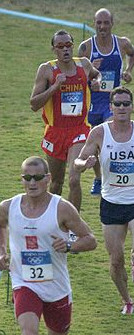
\includegraphics[width=\textwidth]{./figure/Pentathlon.jpg}
\end{center}
\end{column}
\end{columns}
\end{frame}

%%%%%%%%%%%%%%%%%%%%%%%%%%%%%%%%%%%%%%%%
\begin{frame}{Il significato del teorema di Arrow dal punto di vista politico}
Sul piano dei processi decisionali democratici
\begin{itemize}
\item La democrazia è impossibile (!)
\item Non esiste un modo ovvio e privo di ambiguità/problemi di aggregare le
preferenze individuali
\item In che misura il processo democratico è riducibile a un algoritmo per
aggregare preferenze date a priori?
\begin{itemize}
\item Confronto dei diversi argomenti
\item Necessità di rifarsi in modo coerente a criteri fondamentali condivisi
\end{itemize}
\end{itemize}

\begin{quotation}
\linespread{.9}\noindent\footnotesize La necessità di raggiungere un accordo costringe ciascun partecipante a tenere conto del punto di vista degli altri e ad avanzare proposte in termini di principi generali e considerazioni politiche che risultino accettabili per gli interlocutori. Anche se inizialmente il mio obiettivo è quello di sostenere le ragioni particolari del gruppo cui appartengo o che rappresento, nella discussione non posso semplicemente dire «Ritengo che il gruppo A -- gli agricoltori o i poliziotti -- debba avere più soldi». Devo fornire ragioni per questa richiesta. Queste possono essere che il gruppo in questione ha necessità particolari, o che è nell'interesse di tutti migliorare le condizioni di vita del gruppo. Fornendo tali ragioni, mi vincolo al principio generale, che di conseguenza dovrò applicare anche ad altri gruppi che si trovino in condizioni simili.
\end{quotation}
\end{frame}

%%%%%%%%%%%%%%%%%%%%%%%%%%%%%%%%%%%%%%%%
\begin{frame}{Il significato del teorema di Arrow per l'economia del benessere}
Sul piano dell'analisi economica del benessere
\begin{itemize}
\item Non è possibile dedurre un ordinamento di preferenza collettivo rispetto ad
un insieme $X$ di alternative (funzione di benessere sociale) dalle
preferenze individuali
\item in realtà (Sen) questa impossibilità nasce dal fatto che la base per
valutare i benefici individuali è data dalle preferenze, che ipotizziamo
\emph{ordinali} e \emph{non confrontabili}---tale base informativa è insufficiente
\item gli economisti utilizzano comunque la funzione di benessere sociale come
strumento analitico: ciò equivale ad assumere implicitamente che i confronti
interpersonali siano possibili
\end{itemize}
\end{frame}
\end{document}